%Version 3.1 December 2024
% See section 11 of the User Manual for version history
%
%%%%%%%%%%%%%%%%%%%%%%%%%%%%%%%%%%%%%%%%%%%%%%%%%%%%%%%%%%%%%%%%%%%%%%
%%                                                                 %%
%% Please do not use \input{...} to include other tex files.       %%
%% Submit your LaTeX manuscript as one .tex document.              %%
%%                                                                 %%
%% All additional figures and files should be attached             %%
%% separately and not embedded in the \TeX\ document itself.       %%
%%                                                                 %%
%%%%%%%%%%%%%%%%%%%%%%%%%%%%%%%%%%%%%%%%%%%%%%%%%%%%%%%%%%%%%%%%%%%%%

%%\documentclass[referee,sn-basic]{sn-jnl}% referee option is meant for double line spacing

%%=======================================================%%
%% to print line numbers in the margin use lineno option %%
%%=======================================================%%

\documentclass[lineno,pdflatex,sn-mathphys-num]{sn-jnl}% Math and Physical Sciences Numbered Reference Style

%%=========================================================================================%%
%% the documentclass is set to pdflatex as default. You can delete it if not appropriate.  %%
%%=========================================================================================%%

%%\documentclass[sn-basic]{sn-jnl}% Basic Springer Nature Reference Style/Chemistry Reference Style

%%Note: the following reference styles support Namedate and Numbered referencing. By default the style follows the most common style. To switch between the options you can add or remove Numbered in the optional parenthesis.
%%The option is available for: sn-basic.bst, sn-chicago.bst%

%%\documentclass[pdflatex,sn-nature]{sn-jnl}% Style for submissions to Nature Portfolio journals
%%\documentclass[pdflatex,sn-basic]{sn-jnl}% Basic Springer Nature Reference Style/Chemistry Reference Style
%%\documentclass[pdflatex,sn-mathphys-ay]{sn-jnl}% Math and Physical Sciences Author Year Reference Style
%%\documentclass[pdflatex,sn-aps]{sn-jnl}% American Physical Society (APS) Reference Style
%%\documentclass[pdflatex,sn-vancouver-num]{sn-jnl}% Vancouver Numbered Reference Style
%%\documentclass[pdflatex,sn-vancouver-ay]{sn-jnl}% Vancouver Author Year Reference Style
%%\documentclass[pdflatex,sn-apa]{sn-jnl}% APA Reference Style
%%\documentclass[pdflatex,sn-chicago]{sn-jnl}% Chicago-based Humanities Reference Style

%%%% Standard Packages
%%<additional latex packages if required can be included here>

\usepackage{graphicx}%
\usepackage{multirow}%
\usepackage{amsmath,amssymb,amsfonts}%
\usepackage{amsthm}%
\usepackage{mathrsfs}%
\usepackage[title]{appendix}%
\usepackage{xcolor}%
\usepackage{textcomp}%
\usepackage{manyfoot}%
\usepackage{booktabs}%
\usepackage{algorithm}%
\usepackage{algorithmicx}%
\usepackage{algpseudocode}%
\usepackage{listings}%
\usepackage{url}%
%%%%

%% as per the requirement new theorem styles can be included as shown below
\theoremstyle{thmstyleone}%
\newtheorem{theorem}{Theorem}%  meant for continuous numbers
%%\newtheorem{theorem}{Theorem}[section]% meant for sectionwise numbers
%% optional argument [theorem] produces theorem numbering sequence instead of independent numbers for Proposition
\newtheorem{proposition}[theorem]{Proposition}%
%%\newtheorem{proposition}{Proposition}% to get separate numbers for theorem and proposition etc.

\theoremstyle{thmstyletwo}%
\newtheorem{example}{Example}%
\newtheorem{remark}{Remark}%

\theoremstyle{thmstylethree}%
\newtheorem{definition}{Definition}%

\raggedbottom

\begin{document}

\title[Measuring Technological Complexity Using Japanese Patents]{Measuring Technological Complexity Using Japanese Patents}

\author*[1]{\fnm{Rintaro} \sur{Karashima}}
\email{rintaro.karashima@gmail.com}
\equalcont{These authors contributed equally to this work.}

\author[1,2]{\fnm{Hiroyasu} \sur{Inoue}}
\equalcont{These authors contributed equally to this work.}

\affil*[1]{\orgdiv{Graduate School of Information Science}, \orgname{University of Hyogo}, \orgaddress{\street{7-1-28 Minatojima-minamimachi, Chuo-ku}, \city{Kobe}, \postcode{650-0047}, \state{Hyogo}, \country{Japan}}}

\affil[2]{\orgdiv{Center for Computational Science}, \orgname{RIKEN}, \orgaddress{\street{7-1-26 Minatojima-minamimachi, Chuo-ku}, \city{Kobe}, \postcode{650-0047}, \state{Hyogo}, \country{Japan}}}

\abstract{Patent-based measures of technological complexity are widely used to assess technological capabilities, but they are usually computed over regions, and it remains unclear what is gained when corporations replace regions as the unit of analysis.
We compute the Technological Complexity Index (TCI), a network-based measure of technological sophistication, at the corporate level from Japanese patents filed in fiscal years 1981 to 2010, and compare it head-to-head with a regional counterpart derived from the same data on a bipartite network of 1,936 corporations and technology classes at granularities of 35 and 124 classes.
The corporate rankings are less sensitive to the refinement of the classification, but a subsampling analysis shows that most of this advantage reflects the larger number of actor nodes rather than the corporate level itself.
Estimating TCI directly from networks restricted to individual prefectures also fails, because the estimates degenerate for smaller prefectures.
In an out-of-sample test, however, corporate TCI computed on the national network and attributed to prefectures predicts which technologies prefectures newly enter after the study period, whereas regional TCI does not, and this advantage appears only at fine classification granularity.
These results indicate that the value of corporate level measurement lies in the information it preserves at fine granularity, and they provide practical guidance for applying complexity measures to subnational units.}

\keywords{Technological Complexity Index, Japanese patents, corporate level analysis, method of reflections, bipartite networks, economic complexity}

\maketitle

\section{Introduction}\label{section:Introduction}

Technological capability is widely recognized as a key determinant of national competitiveness and economic growth \cite{EC_SSP_nodate,Teixeira2022,NISTEP_nodate}.
Understanding and measuring such capability is therefore essential for analyzing the sources of innovation and designing effective industrial and science policies \cite{gault2023handbook}.

Historically, technological capability has been assessed using quantitative indicators derived from bibliographic data such as patents and publications.
These include measures based on counts of outputs as well as citation-based indicators that incorporate information on technological impact and diffusion \cite{jaffe2019patent,aristodemou2018citations}.
While these indicators provide useful insights into the production and influence of knowledge, they primarily evaluate individual inventions or outputs.
As a result, they do not capture how technological capabilities are structured across actors and technological fields.
Understanding such structure requires moving beyond individual outputs to consider how actors are connected to technologies.

Technological capabilities emerge from interactions between economic actors, such as regions and corporations, and the technologies they develop and combine \cite{katz2016complex}.
These interactions form structured patterns that reflect how capabilities are distributed across actors and technologies.
Empirical studies have shown that such patterns often exhibit nested structures, in which broadly capable actors participate in both common and rare technologies, while more specialized actors tend to be active primarily in ubiquitous technologies \cite{hidalgo2009eci, ren2020bridging}.
Such nested structures reflect differences in the underlying capabilities required to produce technologies.
Understanding this structure is essential for identifying the key technologies and actors that shape technological capability and for developing effective science and technology strategies.
However, because these systems are organized through complex and structured interactions, identifying such key elements remains difficult.

The method of reflections \cite{hidalgo2009eci} provides a framework for addressing this limitation by jointly considering the diversity of actors and the ubiquity of technologies.
This approach enables the quantification of economic and technological complexity and reveals structural patterns that are not captured by conventional indicators.
Building on this framework, a growing body of research has developed alternative complexity measures and extended the approach to different domains \cite{Hidalgo2021,Hidalgo2023,Hausmann2024,Balland2022,diodato2024handbook}.
In particular, Balland and Rigby pioneered the application of this methodology to patent data by measuring the complexity of knowledge produced in US metropolitan areas \cite{balland2017tci}.
Subsequent studies have extended patent-based complexity analysis to European regions \cite{Pinheiro2022,ballandandboschma2021} and to Asian economies \cite{Abay2024}.
Related work has measured patent-based fitness and complexity at the urban scale \cite{straccamore2023urban} and has compared technological fitness and coherence across geographical scales \cite{straccamore2025comparative}.
In parallel, complexity-related constructs such as fitness, coherence, and relatedness have been applied to micro-level actors, including firm--product networks \cite{Bruno2018,Buccellato2016}, corporate technological portfolios and their coherent diversification \cite{pugliese2019coherent}, and a firm-level application of TCI to Korean corporations \cite{Jun2023}.

Despite these advances, most patent-based complexity studies have used regions or countries as the unit of analysis \cite{Hidalgo2021}.
Micro-level complexity measurement is therefore not new in itself, and the firm-level studies cited above have mainly examined how individual firms diversify their portfolios or how firm-level indices behave.
Comparisons across levels of aggregation have so far focused on geographical scales for patent data \cite{straccamore2025comparative} and on the contrast between companies and countries for export data \cite{laudati2023different}.
A firm-level TCI has also been computed for Korean corporations to study sectoral technological leadership \cite{Jun2023}, but that study does not compare the corporate measurement with a regional counterpart.
By contrast, a direct comparison between regional and corporate actors on the same patent data within a single country has received little attention.
Technological capabilities ultimately arise from the activities of corporations that develop, combine, and apply technologies.
Our study therefore differs from prior patent-complexity studies in four respects.
First, the unit of analysis is the corporation, which replaces the region as the actor side of the bipartite network while the technology side remains identical.
Second, the metric is the standard TCI derived from the method of reflections, and we do not propose a new index, which enables a like-for-like comparison between corporate-level and regional-level estimates.
Third, the empirical question concerns the measurement itself, that is, whether the differences between the two levels reflect the corporate level as such or simply the larger number of actor nodes, and whether the corporate estimates carry information that the regional estimates do not.
Fourth, the substantive contribution is a diagnosis of when corporate-level measurement helps and when it fails, together with an out-of-sample test in which corporate TCI attributed to prefectures predicts new regional technological entries while regional TCI does not.

Our study applies the method of reflections to an extensive set of Japanese patent records to quantify technological complexity at the corporation level.
By constructing bipartite networks linking corporations to technology classes, we develop a detailed measure of technological sophistication.
Our analysis investigates the relationships between technological complexity, ubiquity, and the average corporate diversity of patent technologies, and clarifies how these indicators should be interpreted at the corporate level.
In our data, the corporate-level TCI is less sensitive than the regional-level TCI to the refinement of the technology classification, and a subsampling analysis shows that most of this difference is driven by the number of actor nodes rather than by the corporate level itself.
We then ask whether the corporate estimates nevertheless carry regional information.
Estimating TCI directly from prefecture-restricted networks fails, because the estimates degenerate for smaller prefectures and the differences between prefectures are indistinguishable from a placebo null.
In an out-of-sample test, however, corporate TCI computed on the national network and attributed to prefectures predicts which technologies prefectures newly enter after the study period, whereas regional TCI does not, and this advantage appears only at fine classification granularity.
The analyses from this study provide evidence on the structure and measurement of Japanese technological capabilities, and applications to industrial policy remain a prospect that requires broader validation.

The rest of this paper is organized as follows.
In the Results section, we first characterize the ubiquity, average diversity, and complexity of technological fields, then compare the consistency of corporate and regional evaluations across classification granularities and identify its mechanism, and finally test whether the corporate estimates carry regional information out of sample.
In the Discussion section, we provide a critical analysis of our findings and discuss the implications of our results.
Finally, in the Methods section, we detail the data processing, the construction of the complexity index, the validation procedures, and the robustness checks.

\section{Results}\label{section:Results}

\subsection{Characteristics of Technologies}\label{subsection:characteristics}

In this study, we use the method of reflections to quantify the structural characteristics of technologies based on corporate patent publications from 1,936 corporations filed between fiscal years 1981 and 2010 (see Methods section).
First, we define ubiquity (or degree centrality) $K_{T,0}$ as the number of corporations connected to a technology, where a lower value indicates that the technology is rarer.
Similarly, the average diversity $K_{T,1}$ represents the average number of technological fields covered by the corporations connected to a technology, and its formal definition is given in the Methods section.
A higher value indicates that the technology is developed by corporations with broad technological portfolios, whereas a lower value suggests that it is developed by more specialized corporations.
Generally, the average of each indicator is used as a threshold to distinguish high from low values \cite{hidalgo2009eci,balland2017tci, Balland2018}.

Another key indicator is TCI, which represents the sophistication of a technology as inferred from the structure of the corporation--technology network using the method of reflections.
It is important to note that TCI is not a direct measure of rarity.
The method of reflections assigns a high TCI to a technology when it is developed by corporations whose portfolios are broad and contain other high TCI technologies, so the index summarizes the composition of the corporate base of each technology \cite{hidalgo2009eci,Mealy2019}.
Throughout this paper, we therefore distinguish the rarity of a technology, which is measured by ubiquity $K_{T,0}$, the diversification of the corporations connected to it, which is measured by average diversity $K_{T,1}$, and its sophistication, which is captured by TCI.
Because TCI reflects which corporations develop a technology rather than how many corporations develop it, a technology can be both common and high TCI when it is held mainly by diversified corporations, and rare technologies are not necessarily sophisticated.
Following prior work, we use \(\text{TCI}=0\) as the reference point to distinguish relatively high from low values \cite{balland2017tci}.
Accordingly, we describe technologies with values above the reference point as relatively high TCI and those below it as relatively low TCI.

To systematically evaluate technological characteristics, we map the relationships among ubiquity $K_{T,0}$, average diversity $K_{T,1}$, and TCI across patent technologies (Fig.~\ref{fig:scatter}).
Technologies are classified according to the Schmoch system \cite{Schmoch2008}, as illustrated in Panel A of Fig.~\ref{fig:scatter}. Values for ubiquity and average diversity are normalized by their respective means, while TCI is segmented by the zero threshold.

\begin{figure}[ht]
  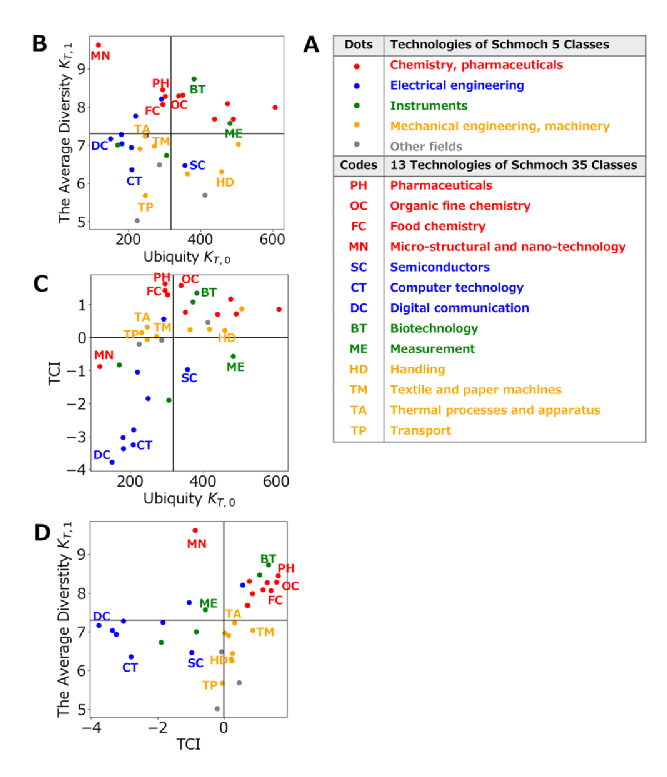
\includegraphics[width=\textwidth]{Figs/Fig1.eps}
  \caption{
  (A) The legend of the five classifications defined by Schmoch \cite{Schmoch2008}, along with an explanation of the technology codes used in Panels (B), (C), and (D).
  (B) The Ubiquity \(K_{T,0}\) versus average diversity \(K_{T,1}\).
  (C) The Ubiquity \(K_{T,0}\) versus TCI.
  (D) The TCI versus average diversity \(K_{T,1}\).
  The black lines in Panels (B), (C), and (D) indicate the mean values of \(K_{T,0}\) and \(K_{T,1}\), and \(\text{TCI} = 0\) is also shown with a black line. Each dot is color-coded according to (A).
  }
  \label{fig:scatter}
\end{figure}

We find a negligible correlation between ubiquity $K_{T,0}$ and average diversity $K_{T,1}$ (Pearson correlation coefficient $r=0.069$), indicating that widely disseminated technologies are not necessarily associated with diversified corporate portfolios (Panel B in Fig.~\ref{fig:scatter}).
We note that this near-zero global correlation is a single summary statistic and does not rule out structured patterns within the panel.
Visual inspection suggests that the technology classes are not scattered at random but cluster by sector, with Chemistry and Pharmaceuticals classes located mainly in the high average diversity region and most Electrical Engineering classes in the low average diversity region, while several Mechanical Engineering classes such as Handling lie in the region of high ubiquity and low average diversity.
The sector-stratified correlations in Fig.~\ref{fig:persector} are consistent with this reading, because the relationships between ubiquity and average diversity within sectors differ from the aggregate pattern.
A test of quadrant concentration points in the same direction without reaching conventional significance, because 23 of the 35 technology classes fall in the high--high or low--low quadrants defined by the mean split, that is 65.7 per cent against about 50 per cent under independence ($\chi^{2}=3.150$, $p=0.076$, $\phi=0.300$).
A fuller quantification of this structure, for example through assortativity measures on the corporation--technology network, is left for future work.

Conversely, ubiquity $K_{T,0}$ and TCI exhibit a moderate positive correlation (Pearson correlation coefficient $r=0.594$), indicating that technologies developed by more corporations tend to receive higher TCI values in this corporate network (Panel C in Fig.~\ref{fig:scatter}).
This pattern is consistent with the interpretation given above, because TCI depends on the portfolios of the connected corporations rather than on rarity itself.
Common technologies held by diversified corporations can therefore rank high, whereas rare technologies held only by specialized corporations rank low.
In this context, Electrical Engineering exhibits low ubiquity, low average diversity, and low TCI values.
This combination indicates that these technologies are developed mainly by corporations that concentrate their innovation efforts within narrowly defined domains.
The low TCI values of this sector should therefore be read as a reflection of this specialized corporate base rather than as a direct statement about the technical difficulty of the field.

Detailed analysis using International Patent Classification (IPC) classes further supports these observations (Fig.~\ref{fig:persector}).
Within the five major sectors defined by Schmoch \cite{Schmoch2008}, the relationship between ubiquity and average diversity is predominantly weak or moderate.
In addition, Electrical Engineering displays a clear positive correlation between ubiquity and TCI (Pearson correlation coefficient $r=0.644$), showing that the positive relationship between ubiquity and TCI observed at the aggregate level is especially pronounced within this sector.

Electrical engineering technologies are predominantly located in the region of low TCI and low average diversity (Panel D in Fig.~\ref{fig:scatter}). In contrast, Chemistry and Pharmaceuticals technologies are clustered in the area of high TCI and high average diversity, exhibiting a positive correlation between these two metrics (Panel D in Fig.~\ref{fig:scatter}, Pearson correlation coefficient $r=0.328$). Furthermore, corporations in the Chemistry and Pharmaceuticals domains are connected not only to fields with low ubiquity but also to those that are more common such as Biotechnology, Analysis of Biological Materials, and Measurement (Panel C in Fig.~\ref{fig:scatter}).
Thus, these results demonstrate a fundamental difference between the two technological domains.
The Chemistry and Pharmaceuticals sectors show high TCI values and are typically developed by corporations with diversified portfolios, whereas Electrical Engineering combines low TCI with a specialized corporate base.
The high TCI of Chemistry and Pharmaceuticals derives from this diversified corporate base rather than from rarity alone, because the corporations in these domains are connected to common fields as well as to rare ones.
A detailed examination reveals a slight negative correlation between ubiquity and average diversity within these sectors (Fig.~\ref{fig:persector}), suggesting that corporations with more comprehensive technological portfolios tend to produce the rarer technologies in these high TCI sectors.
Furthermore, the IPC classes corresponding to Biotechnology and Measurement show high TCI values in fields related to the production of sugar and yeast (C13, A21, C12), drug discovery (A61, C07), and the preservation of these technologies (C07, A23). These findings are consistent with the socio-technical context of the period, particularly reflecting the emergence of drug discovery technologies in the 1980s and 1990s \cite{Sakakibara2014,Nakamura2022}. Moreover, the significant roles of food chemistry and biotechnology during the 1990s and 2000s underscore their contribution to the development of additives that enabled safer food preservation and processing not only in Japan but globally \cite{Bhatia2018,Murakami2024}.

\subsection{Consistency across Classification Granularities and over Time}\label{subsection:consistency}

The preceding section focuses on the corporate TCI over the full period from fiscal year 1981 to 2010 and provides a baseline view of technological characteristics in Japan.
In this section, we compare the corporate-level and regional-level TCIs computed from the same patent data and examine how classification granularity affects the consistency of the resulting technology rankings.
Specifically, we compare results derived from the 35 Schmoch classes and the 124 three-digit IPC classes and quantify the mechanism behind the observed differences.
The question of whether the corporate-level estimates carry regional information is addressed separately in the next section.

The two classification systems share the same technological scope but differ in their level of aggregation.
The Schmoch system includes 35 broad technology classes, whereas the three digit IPC used in this study contains 124 finer classes.
Previous studies on regional technological complexity have reported that using finer classifications tends to make the bipartite network sparse and to reduce the consistency of the calculated indicators \cite{morrison2017economic,Tacchella2012}.
Such inconsistency partly reflects the limited number of regional nodes relative to the number of technology classes.
In regional analyses, several dozen to a few hundred regions such as countries or EU cities \cite{Hidalgo2021,nepelski2020technological} are connected to several hundred or thousand technology classes, which limits the variation in ubiquity across technologies and produces a biased distribution of TCI.
By contrast, corporate analyses involve a much larger number of nodes, often exceeding several thousand corporations, and therefore capture a broader range of ubiquity through the iterative calculation.

These tendencies are reflected in the observed distributions of TCI.
In the regional analysis based on the Schmoch system, 27 out of 35 classes fall within the range of 75 to 100 (Fig.~\ref{fig:detailtci}), indicating that most technologies exhibit similar levels of complexity.
This limited dispersion is consistent with the small number of regional nodes, which comprises only 47 prefectures in Japan.
In contrast, the corporate analysis involves 1,936 corporations, resulting in a denser bipartite network that captures greater heterogeneity in technological capabilities.
Consequently, only 17 classes lie within the same range in the corporate case, while the remaining classes show a wider spread of TCI values across technologies.
This broader dispersion reflects the wider variation in ubiquity available in the corporate network, revealing distinct differences in how frequently each technology appears across corporations.

\begin{figure}[ht]
  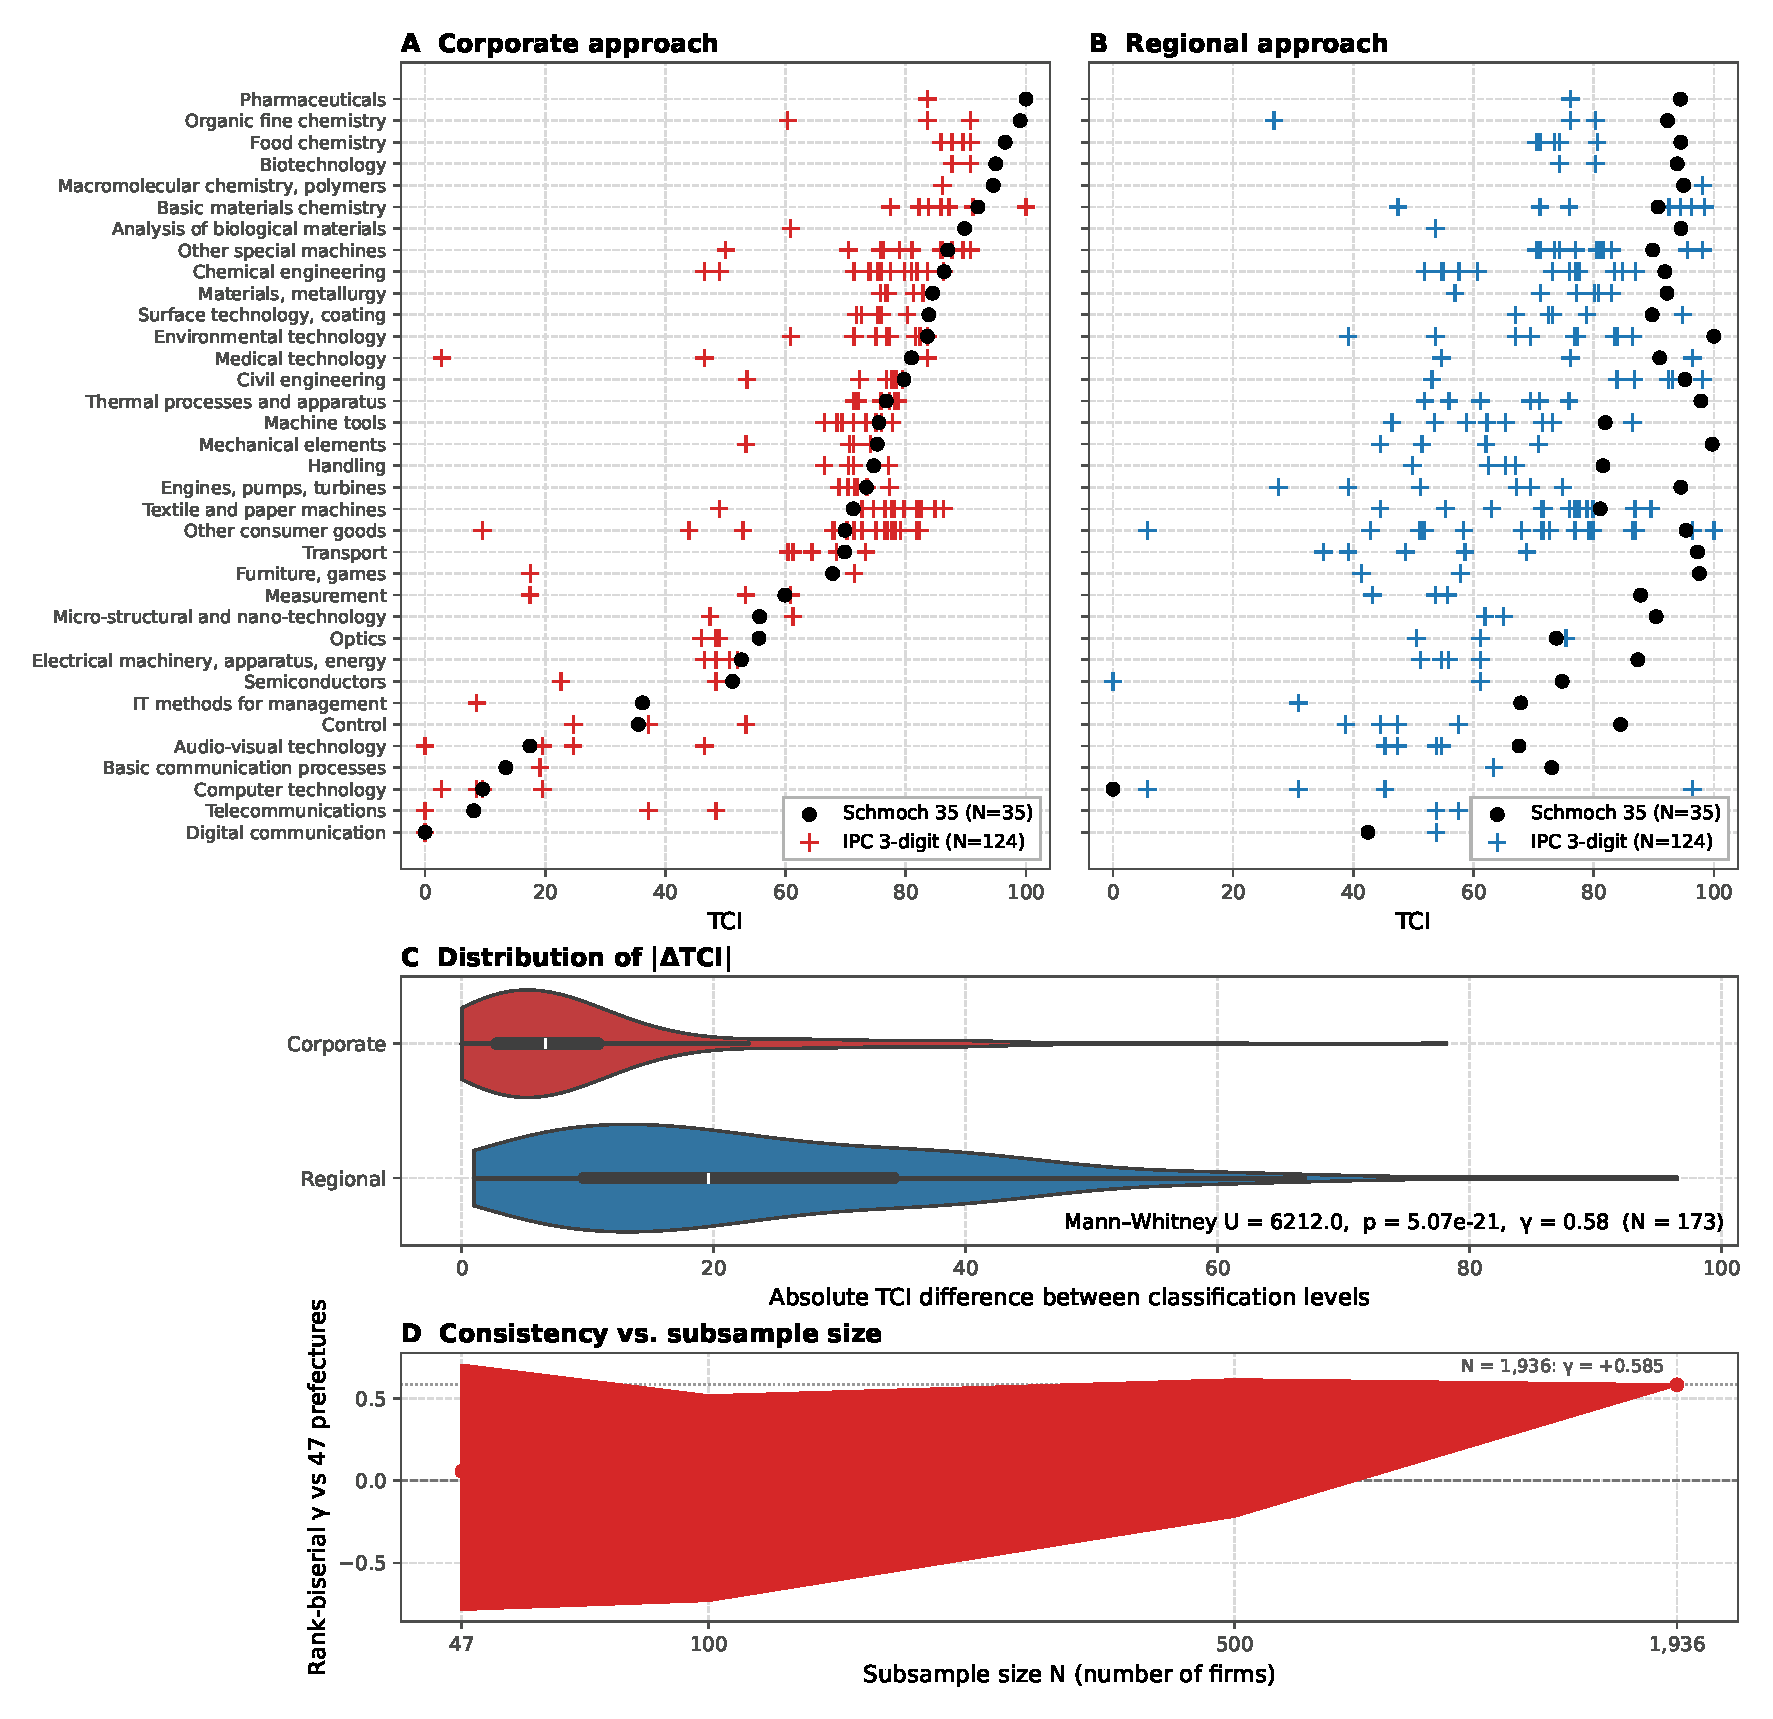
\includegraphics[width=\textwidth]{Figs/Fig2.eps}
  \caption{
    (A) The TCI scores of 124 IPC first three-digit classes and 35 Schmoch classes for the corporate approach.
    For ease of comparison across classifications, TCI values are rescaled to range from 0 to 100 for presentation.
    The midpoint corresponding to \(\mathrm{TCI}=0\) in the original scale is used as the reference when distinguishing relatively high and low values.
    Each IPC is plotted against the corresponding Schmoch axis, and in cases of multiple correspondences, that is, Schmoch class ``Chemical Engineering'' maps to IPC classes B01 to B08, C14, and others, IPC classes are plotted individually.
    (B) The same comparison for the regional approach, using identical axes and rescaling.
    (C) The distribution of the absolute differences between TCI of IPC and of Schmoch classes, for the corporate and regional approaches.
    (D) The median rank-biserial $\gamma$ comparing the corporate and regional residual distributions when the corporate network is subsampled to $N$ corporations, for $N$ = 47, 100, 500, and 1,936.
    Positive values indicate smaller residuals for the corporate analysis.
    The shaded band shows the 5th to 95th percentile range over 100 random subsamples, and the dashed horizontal line marks $\gamma = 0$.
  }
  \label{fig:detailtci}
\end{figure}

The difference between the approaches becomes even clearer when using a finer classification.
When the classification becomes more detailed and the number of technology nodes increases, the regional approach cannot define ubiquity sufficiently.
In the case of Civil engineering, the variance of TCI values for IPC classes corresponding to the same Schmoch class is larger than that for the corporate approach.
The larger difference between the TCI values of the coarse classification and those of the finer classification indicates a greater inconsistency in the evaluation for the regional approach.
A Mann-Whitney U test shows that the distribution of residuals between the TCI values of the Schmoch and IPC classes is significantly different (U = 6212.0, $p$ value = 5.07e-21, $\gamma$ value = 0.585), and that the residuals for the corporate analysis are smaller than those for the regional analysis (Panel C in Fig.~\ref{fig:detailtci}).
The regional TCI in this comparison is computed from the same filtered patent set that the top 3\% criterion retains for the corporate analysis, so the comparison is like for like by construction.
Smaller residuals indicate that, in this dataset, the corporate TCI is less sensitive than the regional TCI to this particular change in classification granularity.
A plausible mechanism is the larger number of actor nodes, because 1,936 corporations provide a richer variation in ubiquity than 47 prefectures and thereby stabilize the iterative calculation.
We test this mechanism directly by recomputing the comparison on random subsamples of corporations of size $N$, with 100 repetitions for each $N$ (Panel D in Fig.~\ref{fig:detailtci}).
When the corporate network is reduced to the same number of actors as the regional network ($N = 47$), the median $\gamma$ drops from 0.585 to 0.057, and the 5th to 95th percentile range spans $-0.783$ to $0.705$ and includes negative values.
The median $\gamma$ rises with the number of actors, reaching 0.116 at $N = 100$, 0.511 at $N = 500$, and 0.585 in the full network with 1,936 corporations.
The median absolute residual shows the same pattern, falling from 18.896 at $N = 47$, which is close to the regional baseline of 19.602, to 6.657 in the full network.
These results indicate that most of the difference observed in Panel C is driven by the number of actor nodes rather than by the corporate level as such, and that the remaining level effect at matched node counts is small and unstable in sign.
The value of the corporate level in this comparison is therefore that it makes a large set of actors available from the same patent data, whereas regional aggregation in Japan is inherently limited to 47 prefectures.

As a complementary view, we also examine five-year rolling TCI rankings based on the 124 IPC classes (SI Fig.~\ref{fig:bump}).
These rolling rankings allow individual technology classes to be followed over time, even though the set of actively filing corporations changes through entry and exit during the period, while corporate reorganizations are consolidated into successor entities as described in the Methods section.
For example, in the IPC classes related to Food Chemistry, a persistently high TCI is observed for sugars (C13) and baking technologies (A21) throughout the 2000s.
By contrast, foodstuffs (A23) and agriculture-related technologies (A01) show gradual declines in ranking, particularly after the mid-1990s.
This suggests that even within related technological fields, some areas maintain their complexity advantage while others lose ground.
We present these trajectories as illustrative observations, and a systematic quantification of the temporal stability of the rankings is left for future work.

\subsection{Regional Information and Out-of-Sample Validation}\label{subsection:validation}

A natural way to use the corporate estimates for regional questions is to restrict the network to the corporations located in each prefecture and to compute TCI separately for each region.
We first show that this direct approach does not work at the sample sizes available here, and then test in a different form whether the corporate estimates carry regional information.
Among the top 3\% corporations, 1,068 are located in Tokyo, 362 in Osaka, and 201 in Aichi.
When TCI is computed on these prefecture-restricted networks, the estimates for Aichi degenerate, with 95.0\% of the technology classes saturating at rescaled TCI values of 95 or above.
The pairwise divergences between prefectures are also indistinguishable from noise.
The median absolute difference in TCI is 4.084 between Tokyo and Osaka (Spearman rank correlation 0.849), 23.271 between Tokyo and Aichi, and 23.712 between Osaka and Aichi.
Against a placebo distribution obtained by pooling the corporations of the three prefectures and randomly reassigning prefecture labels while preserving the actual sample sizes, the observed divergences correspond to the 17.0th, 52.0th, and 48.0th percentiles, and none of them approaches the 95th percentile.
Moreover, the close correspondence between Tokyo and Osaka does not survive when all prefectures are downsampled to the 201 corporations of Aichi, which indicates that this apparent similarity is a product of large samples rather than of similar structures.
We therefore conclude that computing TCI on prefecture-restricted networks is not informative at these sample sizes, and we do not pursue this approach further.

Instead, we test whether the corporate TCI computed on the national network carries information about regional technological development.
We use an out-of-sample design in which all measures are constructed from fiscal years 1981 to 2010 and the outcomes are observed in 2011 to 2015.
The corporate TCI is the same measure as in the preceding sections, computed on the national network of 1,936 corporations, and the regional TCI is computed on the prefecture--technology network from the same patents.
The first outcome is the entry of a prefecture into a technology class, defined as a prefecture--technology pair without revealed advantage in the estimation period that acquires it in the outcome period.
At the three-digit IPC level, there are 4,185 candidate pairs and 366 entries, corresponding to 8.7\% of the candidates.
We estimate logistic regressions of entry on the TCI of the technology class, controlling for prefecture fixed effects, the past RTA of the pair, and the relatedness density of the pair.
Relatedness density is constructed from co-occurrence in the estimation period following the product space literature \cite{hidalgo2007product}, and the identical density variable enters both specifications, so that the corporate and regional specifications differ only in the network on which TCI is measured.

When both TCI variables enter the regression jointly at the three-digit IPC level, the corporate TCI remains a significant predictor of entry while the regional TCI does not.
The standardized coefficient per one standard deviation of TCI is 0.2166 with a 95\% confidence interval of 0.0509 to 0.3823 ($p = 0.0104$) for the corporate measure, and $-0.0938$ with a confidence interval of $-0.2492$ to 0.0616 ($p = 0.237$) for the regional measure (Panel A in Fig.~\ref{fig:validation}).
Relatedness density itself is a strong predictor ($p = 1.9\times10^{-4}$), but including it reduces the corporate TCI coefficient by only about five percent, and density and corporate TCI are nearly orthogonal at this level ($r = 0.023$).
At the Schmoch level of 35 classes, neither measure is significant when entered jointly (corporate $p = 0.223$), although each is significant when entered alone (corporate $p = 0.024$, regional $p = 0.048$).
The value of 0.223 refers to the joint specification without the relatedness density control, and adding the control yields $p = 0.266$ for the corporate measure (Panel A in Fig.~\ref{fig:validation}), so neither measure is significant at this coarse level with or without the control.
The information advantage of the corporate measure therefore appears precisely at the finer classification level, which parallels the granularity pattern documented in the previous section.

We stress that this analysis is an information test rather than a proposal of a prediction tool.
Most of the variation in entry is explained by the prefecture fixed effects, past RTA, and relatedness density, and adding the TCI variables changes the in-sample discrimination only marginally, raising the area under the ROC curve from 0.7974 with the controls alone to 0.7989 with the corporate TCI and 0.7975 with the regional TCI.
The result shows that the corporate TCI contains statistically identifiable information about subsequent regional technological entry that the regional TCI does not, and it does not show that this information is large enough to drive practical forecasting.

As a complementary test on the intensive margin, we regress the log growth rate of each technology's patent share between the estimation and outcome periods on TCI at the three-digit IPC level ($N = 123$), controlling for the log of the past share and for the technology-level average of the relatedness density.
In the joint specification the corporate TCI is significant with a negative sign ($p = 0.0177$) while the regional TCI is not ($p = 0.684$), and this result depends on the density control, because neither measure reaches significance when the two TCI variables are entered jointly without it (Panel B in Fig.~\ref{fig:validation}).
At the Schmoch level neither measure is significant in any of these specifications.
The signs differ between the two outcomes, with high corporate TCI technologies attracting new regional entries while growing more slowly in aggregate patent share.
A possible reading is that the extensive and intensive margins respond differently to complexity, but we treat this contrast as an observation to be explained rather than as an established mechanism.

\begin{figure}[ht]
  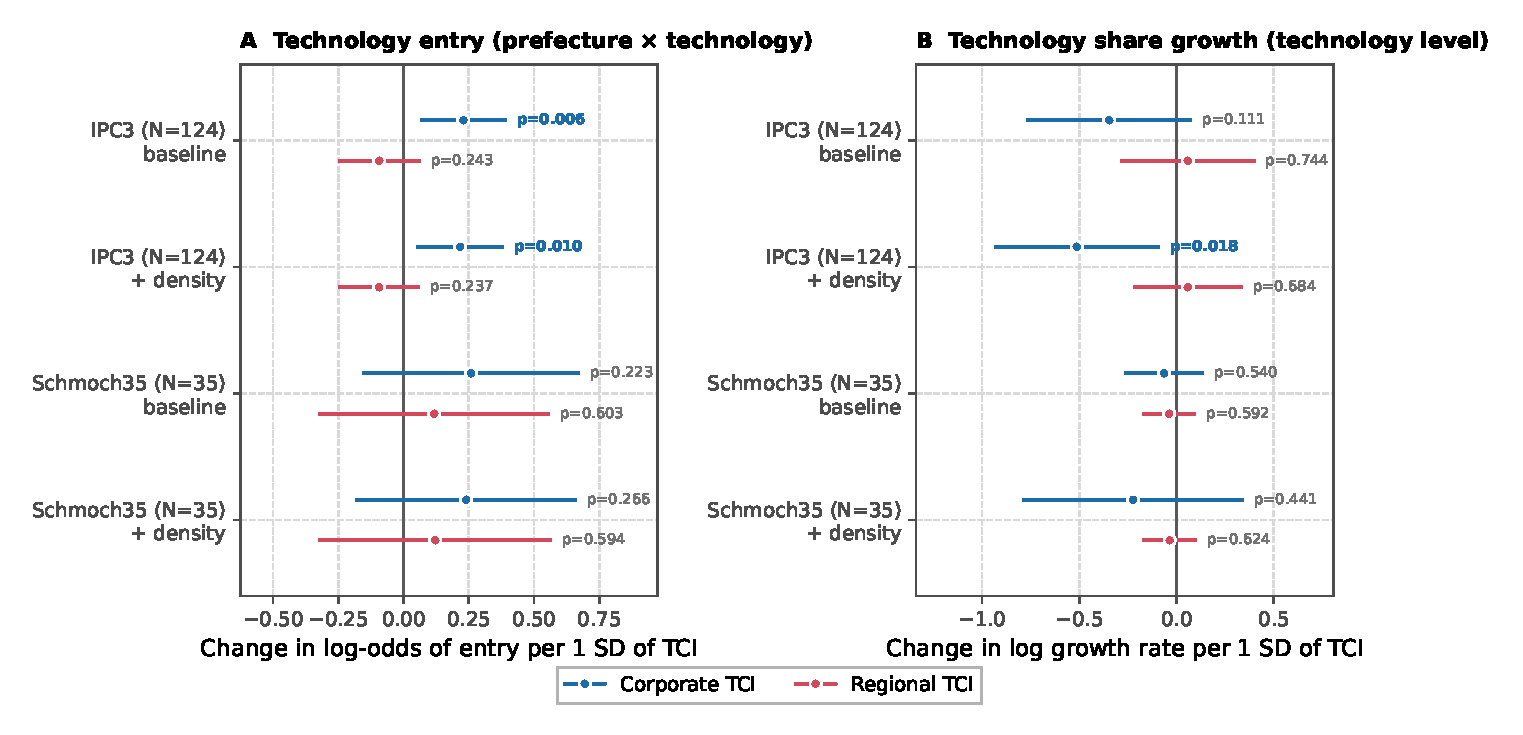
\includegraphics[width=\textwidth]{Figs/Fig3.eps}
  \caption{Out-of-sample comparison of the corporate and regional TCI, with both measures constructed from fiscal years 1981 to 2010 and outcomes observed in 2011 to 2015.
  (A) Standardized logit coefficients of TCI per one standard deviation for the entry of prefectures into technology classes, with 95\% confidence intervals.
  Corporate and regional TCI enter jointly, at the three-digit IPC level and at the Schmoch level, with and without the relatedness density control.
  All specifications include prefecture fixed effects and past RTA.
  (B) Standardized coefficients from the regression of the log growth rate of technology patent shares on TCI, with the same comparison structure.
  Positive coefficients indicate that higher TCI is associated with more entries in Panel A and with faster share growth in Panel B.}
  \label{fig:validation}
\end{figure}

\section{Discussion}\label{section:Discussion}

This study calculates the Technological Complexity Index (TCI) using Japanese patent data to identify sophisticated technologies critical to innovation, and provides three primary contributions.
First, it provides a corporate-level implementation of TCI and compares its behavior with a regional-level counterpart computed from the same patent data.
In this dataset, the corporate-level TCI shows smaller changes in technology rankings than the regional-level TCI when the classification is refined from 35 Schmoch classes to 124 IPC classes.
Our subsampling analysis shows, however, that most of this difference is driven by the number of actor nodes, and that the effect of the corporate level itself is small and unstable in sign once node counts are matched.
The contribution is therefore diagnostic, because it corrects a tempting interpretation and shows that the advantage of the corporate level lies in giving access to a large actor set from the same patent data rather than in an intrinsically more stable measure.
The estimated rankings locate high complexity in the Pharmaceuticals and Chemistry sectors, which agrees with well-documented features of Japanese industrial history during the pharmaceutical industry's formative period \cite{Sakakibara2014,Nakamura2022}.
We regard this agreement as a validation of the corporate-level measurement rather than as a new empirical finding.

Second, the five-year rolling rankings show how temporal trajectories of technologies can be traced within the same framework.
The examples in the Results, such as the persistently high position of sugar-related classes and the gradual decline of foodstuffs and agriculture-related classes, suggest which fields sustained high complexity during Japan's prolonged period of modest economic growth.
We regard this temporal tracing as an illustration of what the corporate-level implementation makes possible rather than as systematic evidence of stable ranking transitions.

Third, for the regional question, we first show that estimating TCI directly from prefecture-restricted networks does not work at this sample size, because the estimates degenerate for smaller prefectures and the pairwise differences are indistinguishable from a placebo null.
We then show in an out-of-sample test that corporate TCI computed on the national network predicts new prefecture and technology entries in 2011 to 2015, whereas regional TCI does not, and that this advantage appears only at fine classification granularity.
This establishes that the corporate estimates carry information about regional technological development that the regional estimates do not, although the gain in discriminative performance is marginal and the result is an information test rather than a forecasting tool.
Both the negative and the positive part of this result provide practical guidance for applying complexity measures to subnational units.

At the same time, there are limits that point to future work.
The subsampling result implies that the consistency comparison in Section 2.2 carries little evidence about the merit of the corporate level once the node-count effect is accounted for, so any claim in favor of corporate-level measurement must rest on the information test in Section 2.3.
Disaggregating the regional side to finer geographic units would be an alternative way to match node counts, but prefecture attribution already rests on registered addresses that are recorded under more than one prefecture for 6.46\% of the retained corporations (Section~\ref{subsection:Data}), so finer disaggregation would compound rather than resolve this source of noise.
That test covers one pair of outcomes in one country and one period, and its scope should not be overstated.
The gain in discriminative performance is marginal, the growth result is significant only with the density control and has the opposite sign to entry, and validations against other outcomes such as R\&D expenditure, productivity, and citation impact remain open.
In addition, the degeneracy of prefecture-restricted estimates means that fine regional description remains out of reach at this sample size, and our positive result concerns prediction rather than description.

Although long aggregation windows improve statistical stability, they may obscure path dependent and dynamic processes in technological development, making it difficult to detect emerging trajectories and transitional phases.
In particular, the role of emerging technologies in shaping subsequent technological development through complexity related mechanisms \cite{juhasz2021explaining} may not be fully visible when long time spans are pooled.
Detecting dynamic shifts therefore requires a balance between longer windows that improve stability and shorter windows that capture emerging fields.

Also, beyond temporal aggregation, additional limitations arise from how the bipartite network is constructed and how complexity is inferred from it.
In particular, constructing the network requires an operational link rule, such as an RCA type criterion or a minimum patent count threshold, but when patent activity is sparse these rules may fail to capture technological engagement accurately and can result in sparse bipartite networks that make complexity estimation unstable \cite{PintarEssletzbichler2022}.
To mitigate this sparsity problem, future work can refine both the link rule and the information carried by each link.
One direction is to move from unweighted to weighted edges that reflect the intensity and impact of inventive activity \cite{ivanova2017economic}.
Citation-based measures are natural candidates, such as raw citations, family normalized citations, or time decayed citations, which may represent technological effort and impact more precisely than simple counts \cite{PintarScherngell2022}.
Another direction is to adopt alternative iterative schemes such as the Fitness Complexity algorithm \cite{Tacchella2012}, which uses non linear iterations to capture structure in sparse settings and may yield more robust rankings \cite{Wu2016,Albeaik2017}.
We computed the Fitness Complexity ranking on the same corporate network, and it does not reproduce the TCI ordering, with a Spearman correlation of $-0.643$ between the two rankings at the Schmoch level (Table~\ref{tab:fitness}).
The two frameworks need not order technologies in the same way, and the rank disagreement by itself does not establish which ordering should be preferred or what each framework measures.
The purpose of this paper is to compare corporate and regional units of analysis using TCI, and a comprehensive evaluation of alternative complexity metrics lies outside its scope and remains a task for future work.

Building on these methodological directions, future research should examine how such refinements affect the robustness and generality of TCI.
External validation is a precondition for any claim that the corporate level TCI is more informative than the regional one, and the entry test in Section 2.3 provides a first validation of this kind.
Broader validation targets include citation-based indicators, alternative weighting schemes, and innovation performance outcomes such as R\&D expenditure, productivity, and forward looking patent impact \cite{sweet2019patent, audretsch2021knowledge, mewes2022technological}.
Predictive modelling is a possible application if such validations accumulate, for example through time series forecasting, representation learning, or graph-based models that directly exploit the bipartite structure \cite{tacchella2023relatedness}.
We emphasize that our validation establishes the presence of information about regional entry rather than a practically useful gain in predictive performance, so these directions remain future work.
Cross regional or national analyses \cite{straccamore2023urban, straccamore2025comparative} can test whether the node-count mechanism and the informational advantage of corporate estimates observed here also appear in other innovation systems, and benchmarking across OECD countries can help evaluate generalizability under different institutional and industrial contexts.
This study advances the corporate level understanding of technological complexity in Japan.
The information test provides a first step, and if broader validations confirm it, the corporate level estimates could inform strategic planning and policy design, although we still present this use as a prospect rather than as an implication of the present results.

\section{Methods}\label{section:Methods}

\subsection{Data}\label{subsection:Data}

The dataset utilized in this study comprises registered patents submitted to the Japan Patent Office (JPO) covering fiscal years 1981 through 2010, encompassing detailed records of 3,189,536 patents filed by 64,457 corporations. Patent records adhere to the International Patent Classification (IPC) system and are further categorized according to the Schmoch classification \cite{Schmoch2008}.

Because corporations undergo mergers, acquisitions, and name changes over the three decades, assignee names are harmonized before the analysis using the correspondence table of the NISTEP corporate name dictionary (version 2023\_1).
Each assignee identifier is resolved iteratively to its final successor entity, so that patents filed under predecessor names are attributed to the successor corporation, and the original name is retained when no successor exists.
Orthographic variations in assignee names, such as historical character forms and differences in the notation of legal entity types, are normalized in the same procedure.
This harmonization reassigns 680,493 patents, corresponding to 21.34\% of all records.
Two properties of this procedure should be noted.
First, the dictionary also reflects name changes that occurred after the study period, so assignees are consolidated under their most recent successor even when the change took place after fiscal year 2010, which is consistent with the design of attributing activity to the surviving legal entity.
Second, parent and subsidiary corporations are not consolidated, so each corporate node in the network represents a harmonized legal entity rather than a corporate group.

The Schmoch system aggregates IPC codes into 35 distinct technological fields, ensuring balanced class sizes and technological consistency, and has been widely applied in previous research \cite{PintarScherngell2022,Balland2018,Whittle2019}. Nevertheless, the granularity of classification substantially influences analytical outcomes. Administrative classifications vary markedly in granularity and international comparability, potentially introducing analytical noise or biases if inadequately managed \cite{Hidalgo2021}. Employing consistent classification schemes, exemplified by the Schmoch system utilized in this study, mitigates such issues by providing balanced and coherent technological categories for robust analyses.

Traditional methods for measuring patent contributions typically employ raw patent counts \cite{balland2017tci,Balland2018,PintarScherngell2022,Pinheiro2022,Whittle2019,Jun2023,Abay2024}. However, such counting methods can lead to overestimation, particularly when patents involve multiple corporations or span multiple technological domains \cite{PintarScherngell2022}. To address potential overestimations, the primary IPC class of each patent is mapped onto the corresponding Schmoch field, with patent value fractionally allocated by equally dividing it among associated corporations and technological fields. This fractional allocation prevents overestimation arising from multi-corporation ownership or cross-domain classifications.

The regional approach evaluates technological complexity as a relative index that reflects regional technological capabilities.
However, this method is sensitive to spatial disparities and tends to yield less stable results when finer classifications such as IPC classes are used, compared to broader classifications like the Schmoch system \cite{PintarEssletzbichler2022}.
Such instability appears in both regional and technological complexity evaluations, as it is inherent in the symmetric structure of the underlying bipartite network.
In the regional approach, each patent is attributed to a prefecture through the registered address of the patent holder.
This attribution is subject to noise, because 6.46\% of the retained corporations have addresses recorded under more than one prefecture across the study period, mainly at multi-site firms, and the records do not distinguish formal headquarters relocations from variation in the recorded address.

In this study, we analyze technological complexity at the corporate level to examine whether these limitations can be mitigated and to describe regional technological portfolios in more detail.
Additionally, filtering criteria are essential to exclude extreme cases capable of distorting analytical outcomes \cite{Hidalgo2021,PintarScherngell2022}. Accordingly, a filtering criterion based on patent distribution per corporation is applied in this study, retaining only the top 3\% of corporations in patent output (Fig.~\ref{fig:patentdistribution}). This filtering criterion excludes corporations exhibiting minimal patenting activity, thereby reducing significant analytical noise in network analyses. Following this filtering, the dataset comprises 2,904,188 patents filed by 1,936 corporations, representing approximately 91\% of the original patent volume.
The filter also selects corporations that remain active for most of the study period.
Although 84.6\% of all assignees stop filing before fiscal year 2010, only 154 of the 1,936 retained corporations (8.0\%) do so.
Corporations that stop filing receive no special treatment, because the bipartite network aggregates patents over the whole period.
The corporate nodes in our network can therefore be regarded as largely stable economic actors rather than as a heterogeneous collection of historical assignee records.
Three considerations justify the top 3\% criterion and show that it does not drive our results.
First, the RTA threshold alone provides little pruning, because all 64,457 assignees remain after the RTA step, with a median presence degree of 1, a mean of 2.45, and 57.80\% of corporations connected to a single technology class.
Second, the criterion is defined ex ante on raw patent output and does not condition on the structure of the RTA network from which TCI is computed.
Third, the TCI rankings are robust to the threshold, and alternative pruning rules yield the same or stronger conclusions, as described in Section~\ref{subsection:robustness} (Tables~\ref{tab:threshold} and~\ref{tab:pruning}).

Utilizing these filtered data, technological complexity is based on a bipartite network connecting corporations to technological fields in which they are specialized. Although there are some arguments regarding the optimal specialization index for establishing connections within these networks \cite{PintarScherngell2022}, we follow prior research by employing the Revealed Technological Advantage (RTA) index \cite{Soete1987}.
The RTA index builds upon the revealed comparative advantage framework proposed by Balassa \cite{Balassa1965}.
Specifically, the RTA index for a given corporation in a specific technological field measures the ratio between the share of patents held by corporation \(C\) in technology \(T\) and the share of patents in technology \(T\) among all corporations.
The numerator of the RTA index captures the fraction of patent activity devoted to technology \(T\) for corporation \(C\).
Similarly, the denominator reflects the overall share of patent activity in technology \(T\) among all corporations, computed as the sum of \(W_{CT}\) over all corporations divided by the sum of \(W_{CT}\) over all corporations and technologies.
The RTA index is thus given by

\begin{equation}\label{eq1}
\mbox{RTA}_{CT} = \frac{W_{CT}}{\sum_{T} W_{CT}} \Bigg/ \frac{\sum_{C} W_{CT}}{\sum_{CT} W_{CT}}~.
\end{equation}

We consider that RTA index values of 1 or greater indicate that corporation \(C\) holds a prominent technological advantage in technology \(T\). Based on this threshold, a binary adjacency matrix of the bipartite network \(M_{CT}\) is defined by

\begin{equation}\label{eq2}
M_{CT} =
\begin{cases}
1 & \text{if } \mbox{RTA}_{CT} \geq 1, \\
0 & \text{otherwise}.
\end{cases}
\end{equation}

\subsection{Technological Complexity}\label{subsection:technologicalcomplexity}

The binary matrix \(M_{CT}\) forms the two metrics which characterize each node in the bipartite network by the sum of connections, known as degree centrality. The diversity of corporations \(K_{C,0}\) quantifies the number of technologies in which a corporation is specialized, as indicated by $M_{CT}$.
Similarly, the ubiquity of technologies \(K_{T,0}\) represents the number of corporations that exhibit a technological advantage in a given field. These quantities are computed as

\begin{equation}\label{eq3}
\begin{aligned}
K_{C,0} = \sum_{T} M_{CT},  \\
K_{T,0} = \sum_{C} M_{CT}~.
\end{aligned}
\end{equation}

Higher diversity values indicate corporations with broad technological capabilities, while lower ubiquity values signify that the technologies are rare.
Through calculating these two characteristics of adjacent nodes iteratively, the diversity and ubiquity of each node are updated as

\begin{equation}\label{eq4}
K_{C,N} = \frac{1}{K_{C,0}} \sum_{T} M_{CT}\, K_{T,N-1},
\end{equation}

\begin{equation}\label{eq5}
K_{T,N} = \frac{1}{K_{T,0}} \sum_{C} M_{CT}\, K_{C,N-1}.
\end{equation}

Here, the metric \(K_{T,1}\) represents the average nearest neighbor degree for technology nodes and it reflects the average diversity of corporations connected to a given technology.
Substituting Eq.~(\ref{eq4}) into Eq.~(\ref{eq5}) yields

\begin{equation}\label{eq6}
K_{T,N} = \sum_{T'} \widetilde{M}_{TT'} K_{T',N-2}
\end{equation}

where \(T'\) denotes a technological field, and $\widetilde{M}_{TT'}$ is defined as

\begin{equation}\label{eq7}
\widetilde{M}_{TT'} = \sum_{C} \frac{M_{CT}\, M_{CT'}}{K_{C,0}\, K_{T,0}}~.
\end{equation}

Eq.~(\ref{eq6}) is satisfied when \(K_{T,N} = K_{T,N-2} = 1\), which corresponds to the eigenvector associated with the largest eigenvalue of the stochastic matrix \(\widetilde{M}_{TT'}\).
Since this eigenvector is a vector of ones and not informative, the eigenvector corresponding to the second largest eigenvalue of \(\widetilde{M}_{TT'}\) captures the greatest variance among technology fields \cite{Hidalgo2021, Mealy2019}.
Thus, TCI is given by
\begin{equation}\label{eq8}
TCI = \frac{\widetilde{T} - \langle \widetilde{T} \rangle}{\text{stdev}(\widetilde{T})},
\end{equation}

where \(\widetilde{T}\) represents the eigenvector corresponding to the second largest eigenvalue of \(\widetilde{M}_{TT'}\), and \(\langle \widetilde{T} \rangle\) is their mean and \(\text{stdev}(\widetilde{T})\) is their standard deviation.

\subsection{Robustness Procedures}\label{subsection:robustness}

For the subsampling analysis in Section~\ref{subsection:consistency}, we draw random subsets of corporations of size $N \in \{47, 100, 500, 1936\}$ with 100 repetitions for each $N$ under a fixed random seed.
For each draw, the RTA index is recomputed on the subsample, the bipartite network is rebuilt with the threshold $\mbox{RTA} \geq 1$, and the comparison between the Schmoch and IPC classifications is repeated.
Each draw is summarized by the rank-biserial $\gamma$, and we report the median and the 5th to 95th percentile range across repetitions.

For the filtering threshold, we recompute the full analysis while retaining the top 1, 3, 5, 10, and 100 percent of corporations by patent output, which corresponds to 647, 1,936, 3,232, 6,463, and 64,457 corporations (Table~\ref{tab:threshold}).
The TCI rankings are robust to this choice, because the Spearman correlations with the main specification are at least 0.90 in absolute value for both classifications, and the negative value for the Schmoch classes in the full sample reflects a sign flip of the eigenvector rather than a reversal of the ordering.
The consistency statistic $\gamma$, by contrast, is not monotone in the threshold, taking values of $-0.076$, 0.585, 0.877, 0.576, and 0.721.
The sign reversal at the top 1\% threshold is consistent with the node-count mechanism of Section~\ref{subsection:consistency}, because only 647 corporations remain at that threshold.
The jump at the top 5\% threshold is driven by the regional side, whose median absolute residual deteriorates from 19.6 to 55.7, whereas the corporate side barely moves from 6.66 to 6.85.
The instability of the comparison statistic across thresholds therefore originates mainly from the regional measure, while the corporate rankings themselves remain stable.

We also compare the top 3\% filter with a pruning rule that is more directly motivated by the algorithm, namely removing corporations with a single link after the RTA step (Table~\ref{tab:pruning}).
This rule retains 27,201 corporations and yields $\gamma = 0.962$, which is larger than the 0.585 of our main specification.
This is consistent with the node-count mechanism, because degree-one removal keeps far more corporations than the top 3\% filter.
We nevertheless keep the top 3\% filter as the main specification, because it is defined ex ante on patent output rather than on the network from which TCI is computed, and because the alternative rule would only widen the reported gap, so our main specification is conservative in this respect.

\subsection{External Validation Procedures}\label{subsection:validationprocedures}

For the prefecture-restricted comparison in Section~\ref{subsection:validation}, we construct an independent corporation--technology bipartite network for each prefecture from fiscal years 1981 to 2010 at the three-digit IPC level, using the same $\mbox{RTA} \geq 1$ rule, and rescale TCI to the range from 0 to 100.
Tokyo, Osaka, and Aichi host 1,068, 362, and 201 of the retained corporations.
The placebo test pools the corporations of the three prefectures and randomly reassigns prefecture labels while preserving the observed number of corporations in each prefecture, with 100 repetitions forming the null distribution of the pairwise deviations.
The downsampling check draws random subsets of 201 corporations, which is the size of Aichi, for every prefecture.

For the entry analysis, TCI and all predictors are constructed from fiscal years 1981 to 2010 only, and outcomes are measured in 2011 to 2015.
A candidate is a prefecture and technology pair with $\mbox{RTA} < 1$ in the estimation period, and an entry is defined as a transition to $\mbox{RTA} \geq 1$ in the outcome period.
At the three-digit IPC level, this yields 4,185 candidate pairs, of which 366 (8.7\%) realize an entry.
We estimate logit models with prefecture fixed effects and the past RTA value as controls, and prefectures in which no candidate or every candidate enters are excluded beforehand because they cause complete separation (two prefectures at the IPC level and nine at the Schmoch level).
Coefficients are standardized per one standard deviation of TCI for presentation, which is a linear transformation and leaves the $p$ values unchanged.

The relatedness density control follows the product space approach \cite{hidalgo2007product}.
The proximity $\phi(i,j)$ between two technology classes is the minimum of the two conditional probabilities of their co-occurrence in the presence matrix of the estimation period.
The density of a candidate pair is defined as

\begin{equation}\label{eq9}
\mbox{density}(p,t) = \frac{\sum_{j \neq t} M^{\mbox{\scriptsize pref}}_{pj}\, \phi(t,j)}{\sum_{j \neq t} \phi(t,j)},
\end{equation}

where $M^{\mbox{\scriptsize pref}}_{pj}$ is the prefecture presence matrix of the estimation period.
The same density column enters both specifications, which keeps the head-to-head comparison like for like.
We construct the proximity both from the corporate presence matrix and from the regional presence matrix, and the corporate TCI remains significant in the joint specification in both versions ($p = 0.0104$ and $p = 0.0112$).
In-sample discriminative performance is summarized by the area under the ROC curve and is reported in Section~\ref{subsection:validation}.

For the growth analysis, we regress the log growth rate of each technology's patent share between the estimation and outcome periods on the two TCI variables jointly, controlling for the log of the past share and the technology-level average of the relatedness density, and estimate ordinary least squares with heteroskedasticity-robust standard errors.
At the three-digit IPC level, this yields 123 observations.

\backmatter

\bmhead{Supplementary information}

Three supplementary figures and three supplementary tables are provided in Appendix~\ref{secA1}.
Table~S1 reports the sensitivity of the results to the filtering threshold, Table~S2 compares alternative pruning rules, and Table~S3 compares the TCI and Fitness Complexity rankings of the 35 Schmoch classes.
Fig.~S1 shows the relationships between ubiquity, average diversity, and TCI stratified by Schmoch sector.
Fig.~S2 shows the five-year rolling TCI rankings based on 124 three-digit IPC classes for corporate and regional analyses.
Fig.~S3 shows the diversity distribution of the retained corporations and the concentration of patents among them.

\section*{Declarations}

\textbf{Availability of data and materials:} The patent data utilized in this study were obtained from the Japan Patent Office (JPO) via the J-platPat portal (\url{https://www.j-platpat.inpit.go.jp/}). Records published within the most recent twelve months are directly downloadable. Data older than one year can be provided by the JPO upon reasonable request. Patent classification concordance tables mapping International Patent Classification (IPC) classes to Schmoch technology fields were acquired from the World Intellectual Property Organization (WIPO) IP Statistics portal (\url{https://www.wipo.int/en/web/ip-statistics}).

\textbf{Code availability:} All scripts and code used to compute the Technological Complexity Index and reproduce the results of this paper are publicly available in the following GitHub repository: \url{https://github.com/RintaroKARASHIMA/KCIinJapaneseFirms}.

\textbf{Competing interests:} The authors declare no competing interests.

\textbf{Funding:} This work was supported by Japan Society for the Promotion of Science KAKENHI Grant-in-Aid for Scientific Research (B) Grant Numbers JP25K01454 and JP24K00247, and Watanabe Memorial Foundation for the Advancement of New Technology FY2024 Science and Technology Research Grant Number R6-590. The funders had no role in study design, data collection and analysis, decision to publish, or preparation of the manuscript.

\textbf{Authors' contributions:} H.I. conceived the main research idea, designed the study, collected the data, and secured the funding. R.K. performed the analysis and drafted the manuscript. Both H.I. and R.K. critically reviewed the results, discussed the findings, contributed to the revisions of the manuscript, and approved the final version of the manuscript.

\textbf{Acknowledgements:} This work was supported by Japan Society for the Promotion of Science KAKENHI Grant-in-Aid for Scientific Research (B) Grant Numbers JP25K01454 and JP24K00247, and Watanabe Memorial Foundation for the Advancement of New Technology FY2024 Science and Technology Research Grant Number R6-590. The funders had no role in study design, data collection and analysis, decision to publish, or preparation of the manuscript.

\begin{appendices}

\section{Supplementary Figures and Tables}\label{secA1}

\renewcommand{\thefigure}{S\arabic{figure}}
\setcounter{figure}{0}
\renewcommand{\thetable}{S\arabic{table}}
\setcounter{table}{0}

\begin{figure}[ht]
    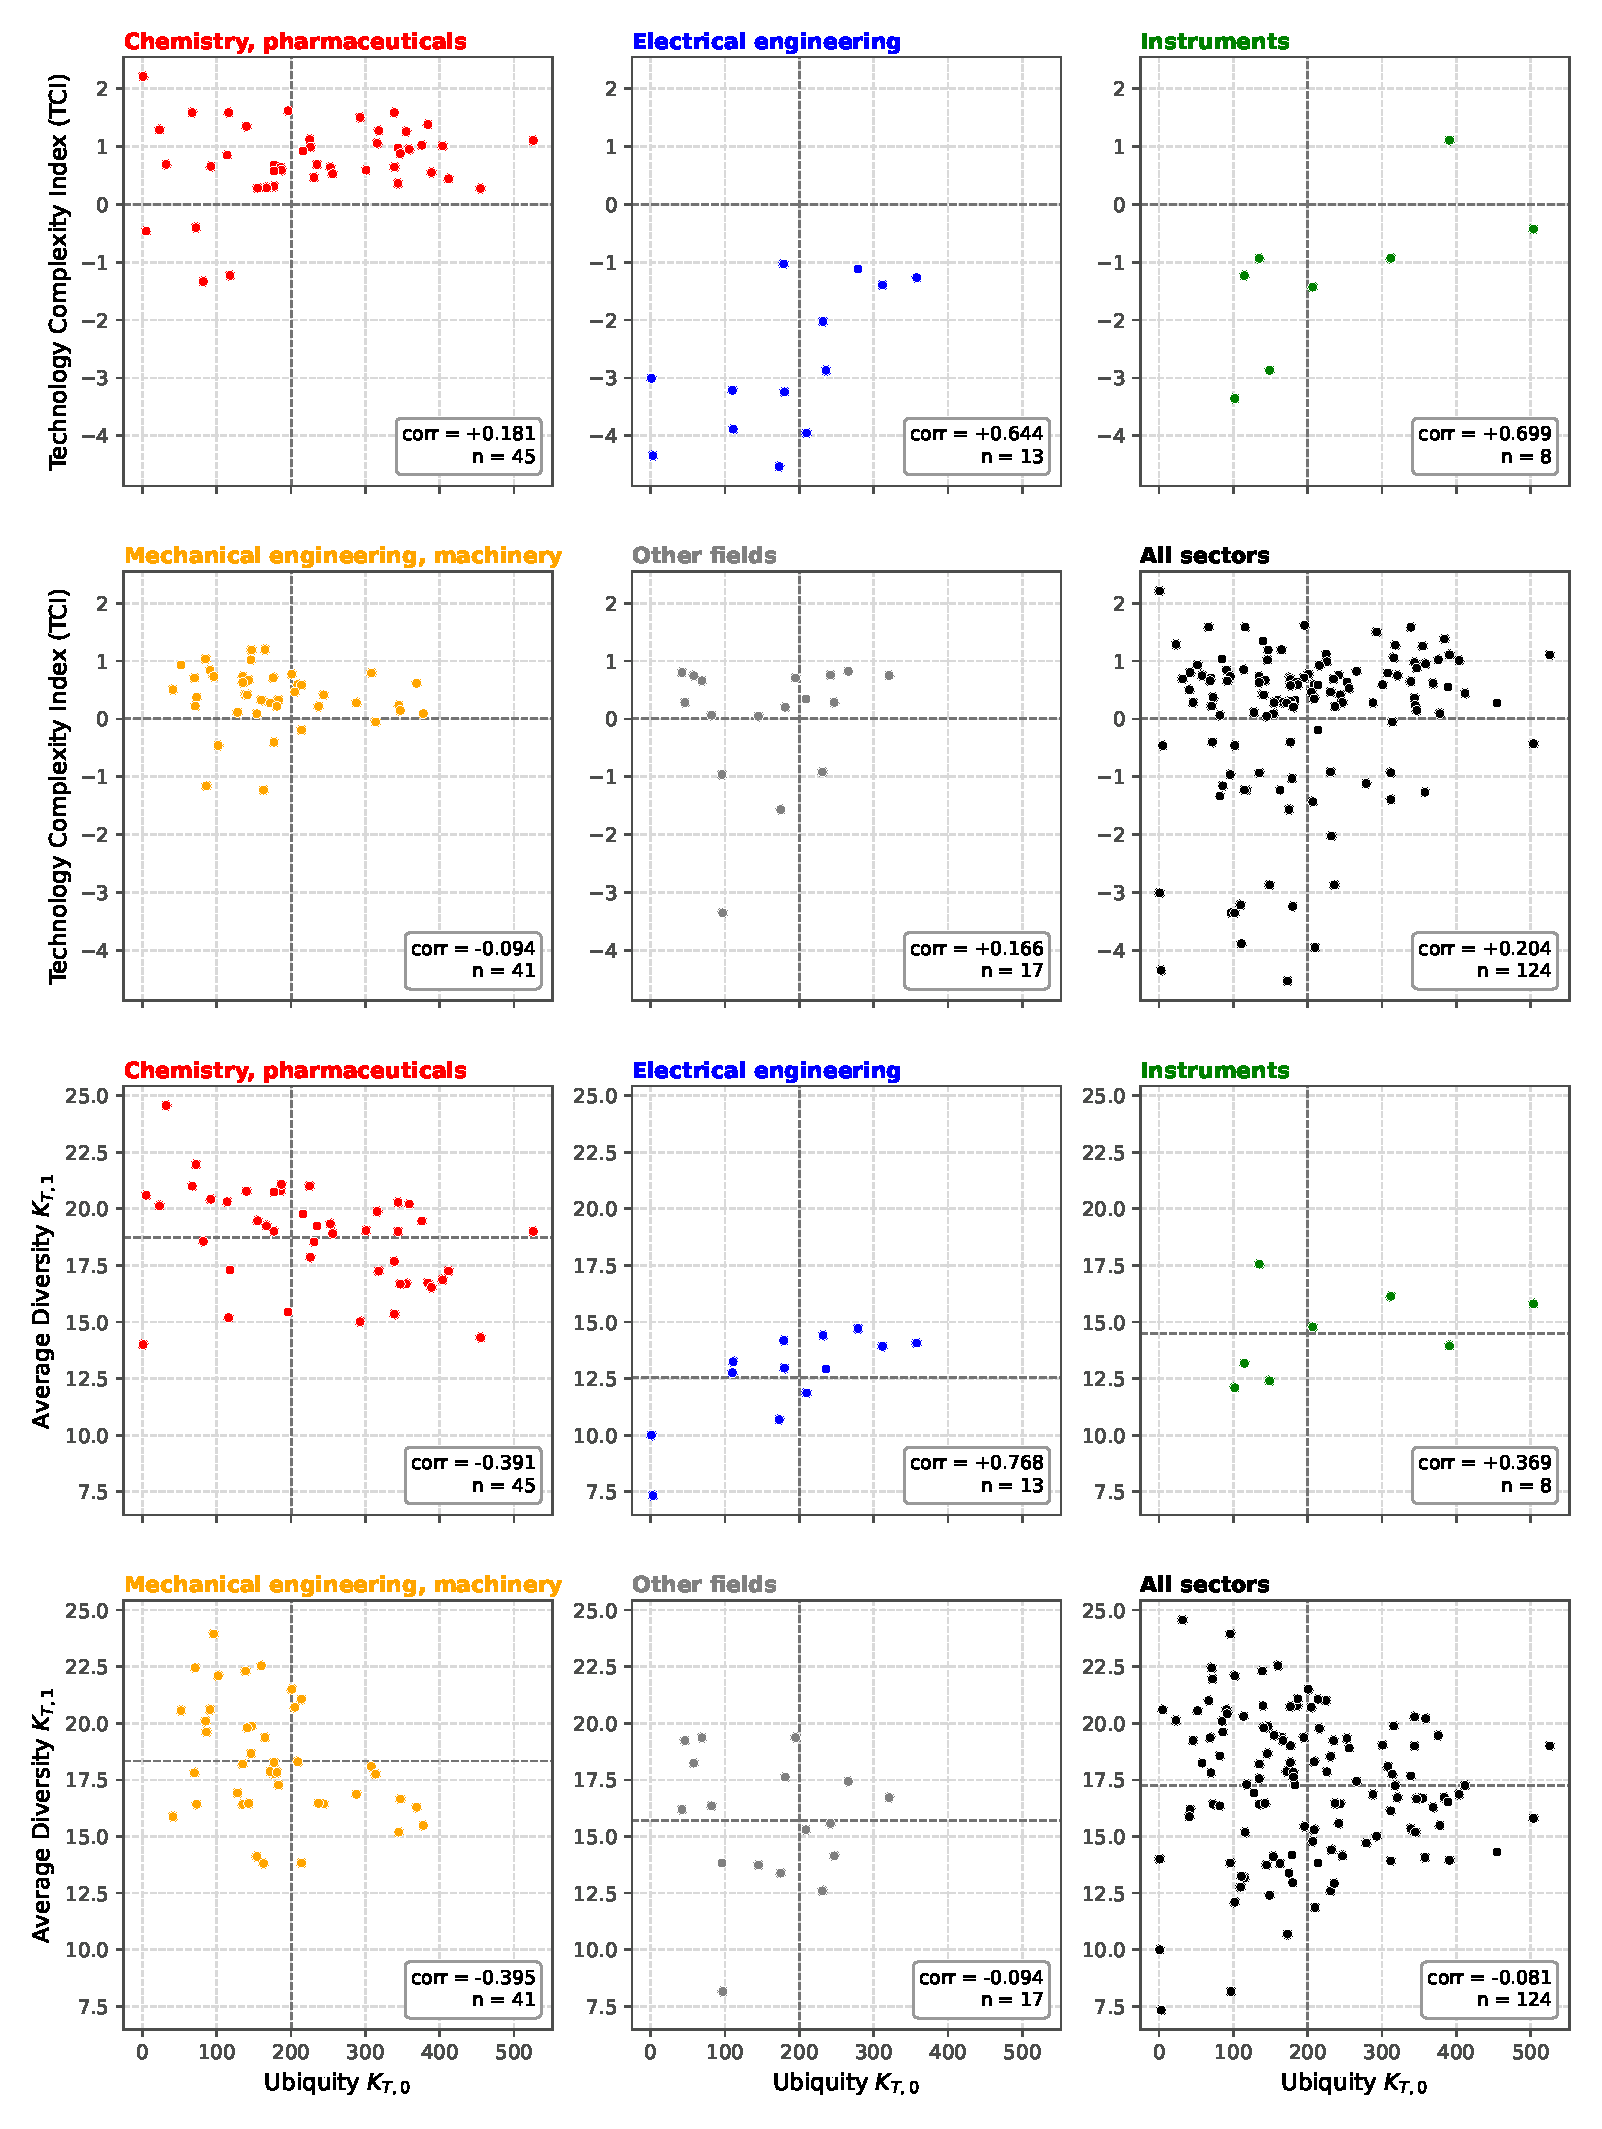
\includegraphics[width=\textwidth]{Figs/FigA1.eps}
    \caption{The relationship between the ubiquity \( K_{T,0} \) of a technology node \( T \) and two other node quantities, based on the 124 three-digit IPC classes.
      The upper two rows show TCI against ubiquity, and the lower two rows show the average nearest neighbor degree \( K_{T,1} \) against ubiquity.
      Within each block, five panels stratify the classes by the five sectors defined by Schmoch \cite{Schmoch2008} and the sixth panel pools all sectors.
      The dashed lines indicate the mean value on each axis, and the annotation in each panel reports the Pearson correlation and the number of classes.}
    \label{fig:persector}
\end{figure}

\begin{figure}[ht]
    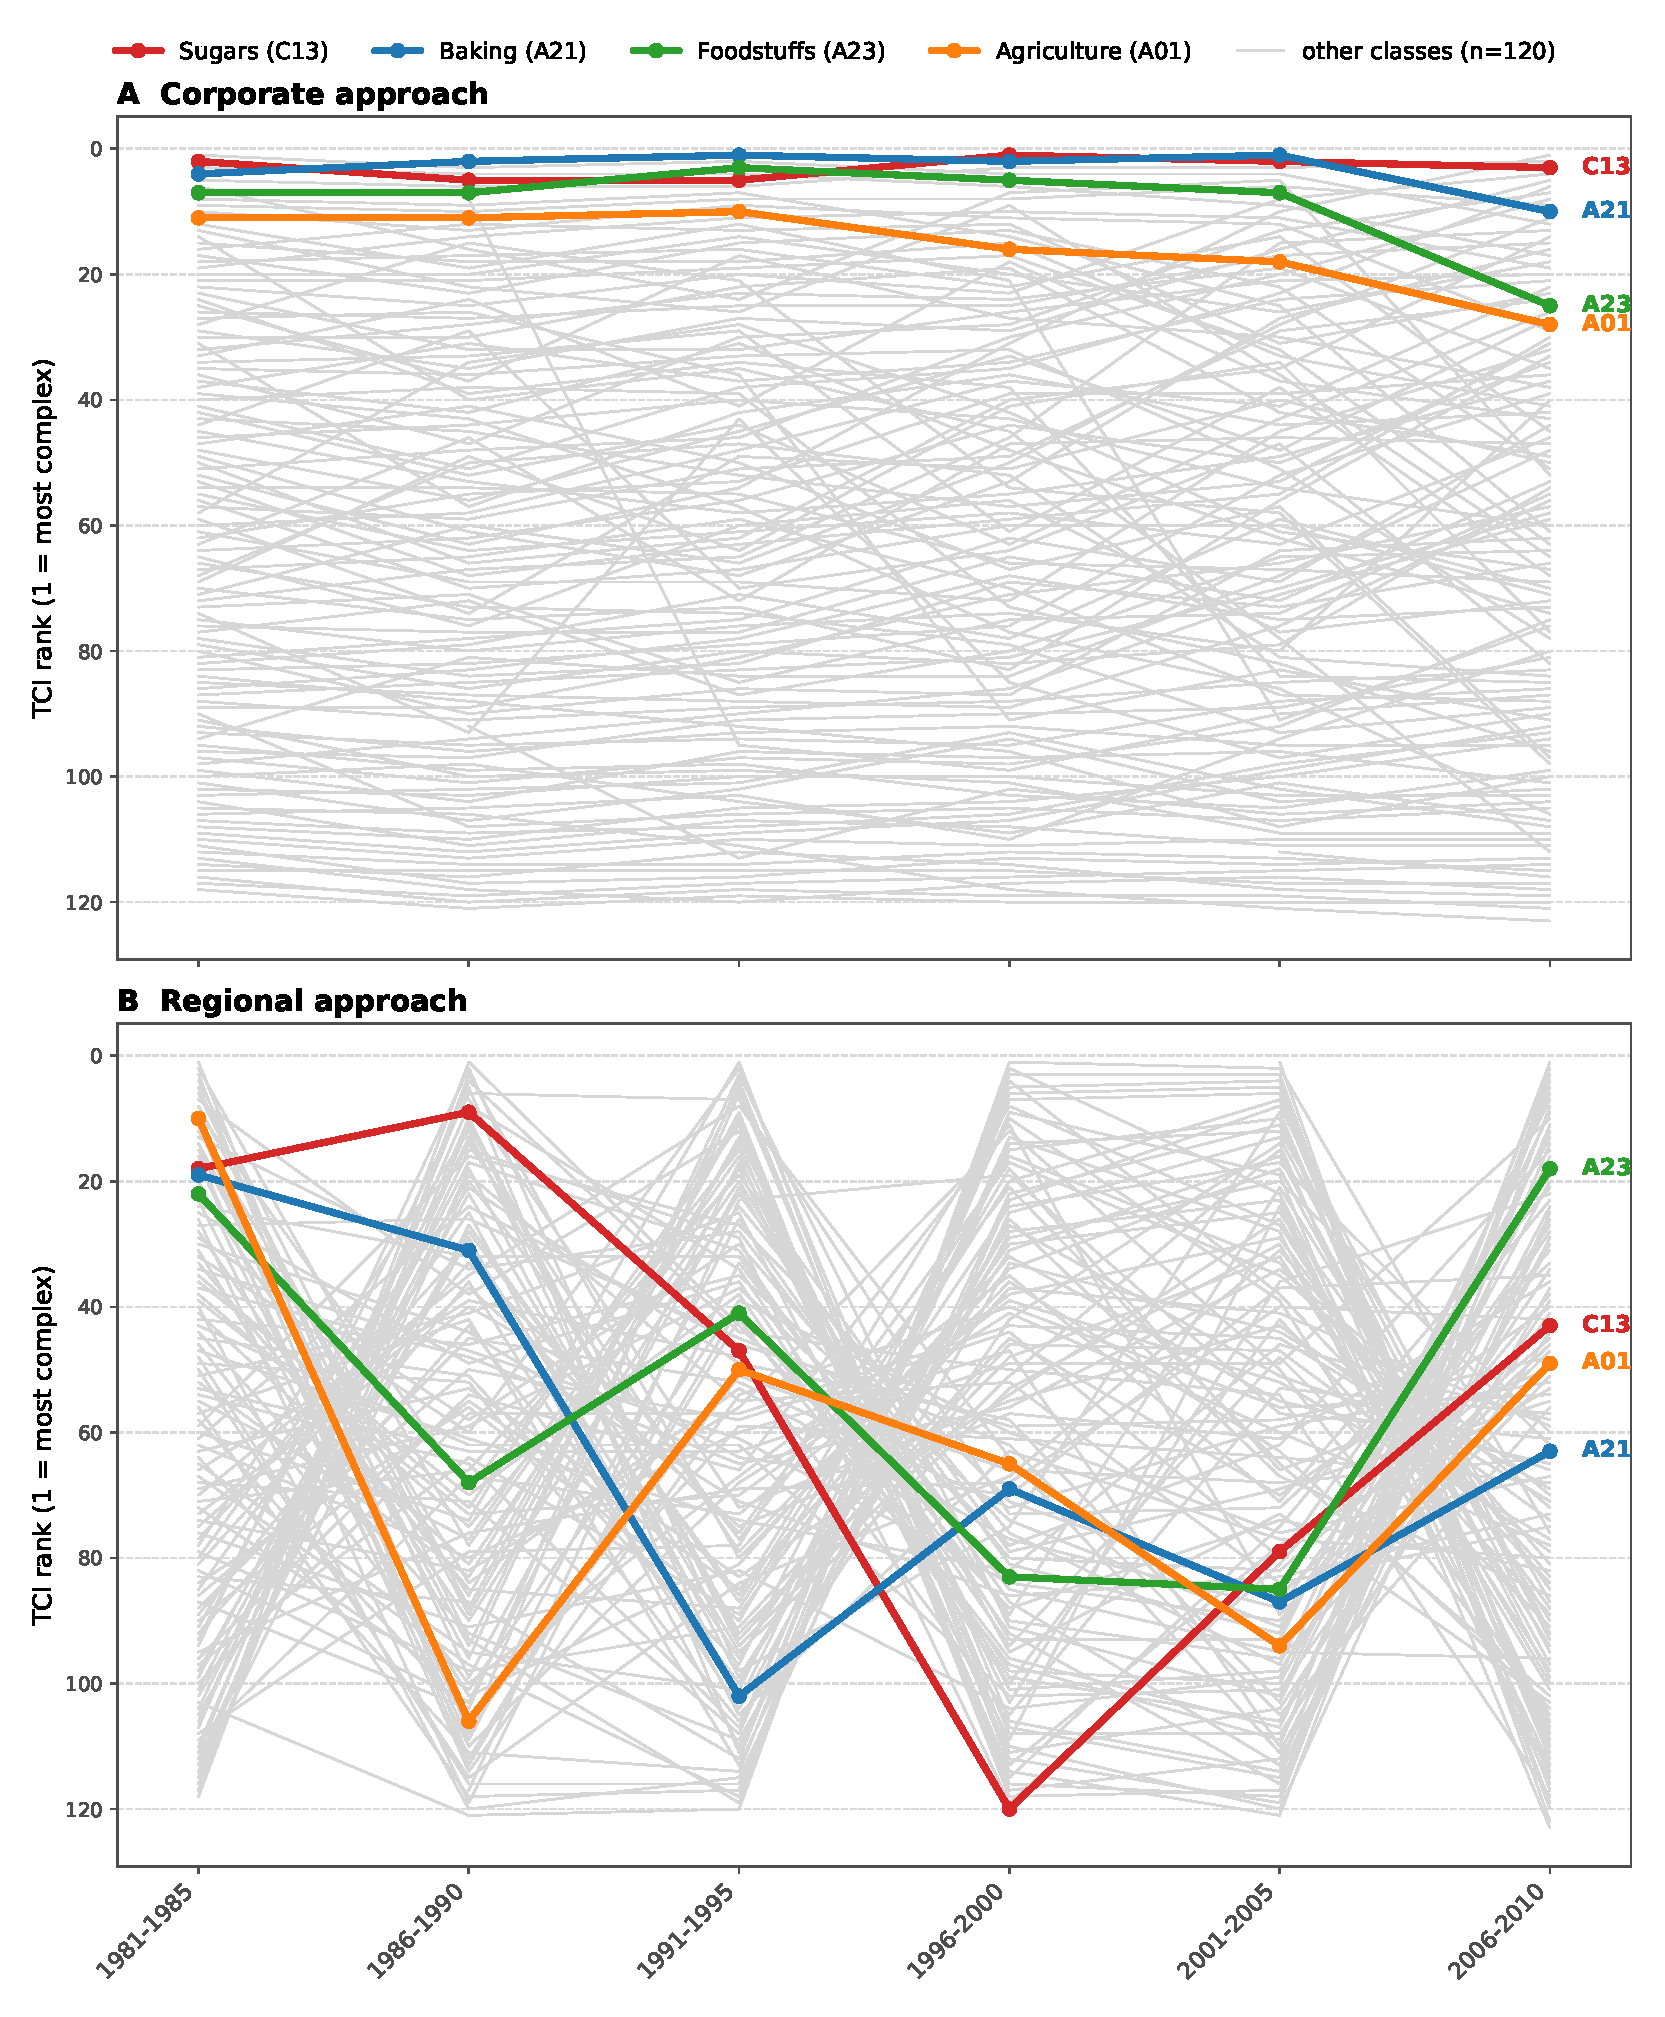
\includegraphics[width=\textwidth]{Figs/FigA2.eps}
    \caption{Changes in the five-year rolling ranking of the TCI based on 124 three-digit IPC classes for
      (A) the corporate analysis and
      (B) the regional analysis.
      The four classes interpreted in the main text are drawn in color with end point labels, and the remaining 120 classes are drawn in light gray to give an overview of all 124 trajectories.
      These classes are sugars (C13) and baking technologies (A21), which show persistently high TCI in the corporate ranking, and foodstuffs (A23) and agriculture-related technologies (A01), which decline gradually after the mid-1990s.
    }
    \label{fig:bump}
\end{figure}

\begin{figure}[ht]
    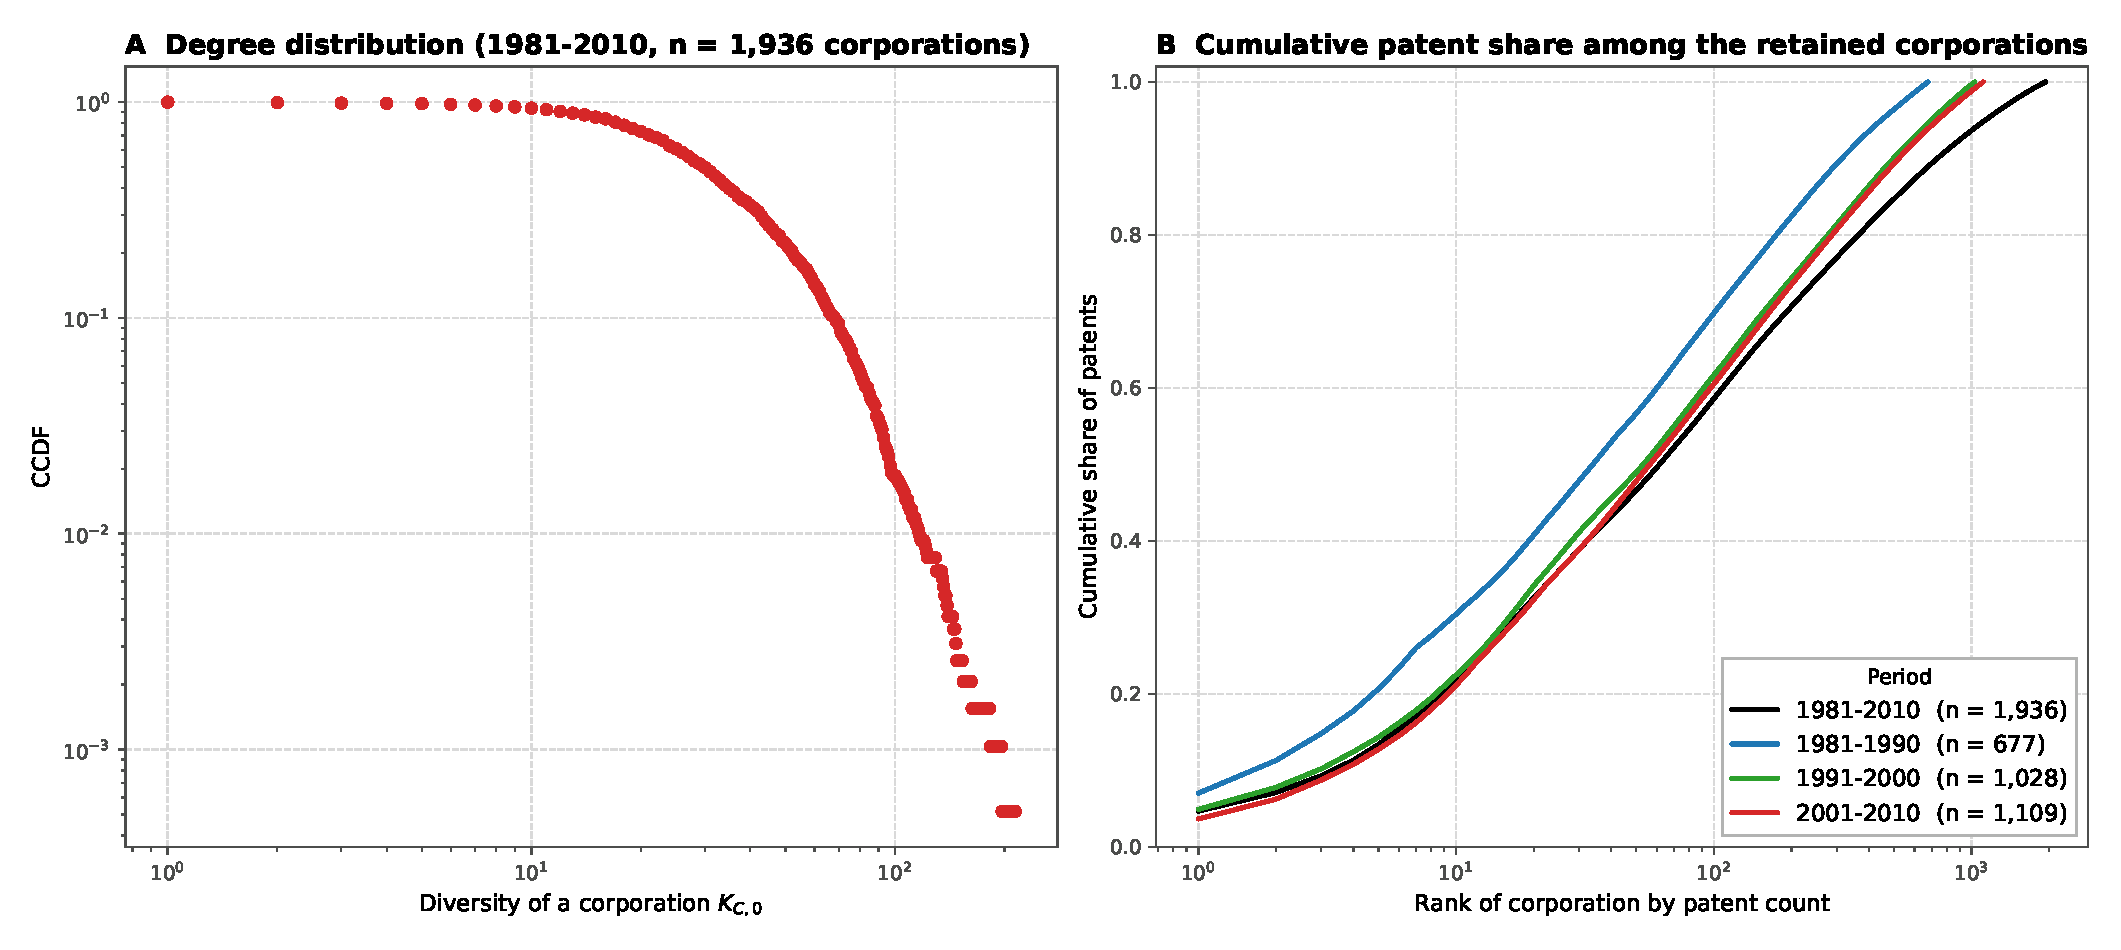
\includegraphics[width=\textwidth]{Figs/FigA3.eps}
    \caption{(A) The complementary cumulative distribution function (CCDF) of the diversity \( K_{C,0} \) of the 1,936 corporations retained by the top 3\% filter, computed over fiscal years 1981 to 2010.
      (B) The cumulative share of patents among the retained corporations against their rank by patent count, shown for the whole period and separately for each of the three decades.
      Both panels describe the corporations that remain after filtering, and the retained set accounts for approximately 91\% of all patents.}
    \label{fig:patentdistribution}
\end{figure}

\begin{table}[ht]
\caption{Sensitivity of the results to the filtering threshold.
Corporations are retained by the top $p$ percent of patent output.
Spearman correlations compare the TCI ranking under each threshold with the main specification ($p = 3$).
The rank-biserial $\gamma$ compares the corporate and regional residual distributions as in Fig.~\ref{fig:detailtci}.
The negative Spearman correlation for the Schmoch classes at $p = 100$ reflects a sign flip of the eigenvector rather than a reversal of the ordering.}
\label{tab:threshold}
\begin{tabular}{lrrrr}
\toprule
Threshold $p$ (\%) & Corporations & $\rho$ (Schmoch) & $\rho$ (IPC) & $\gamma$ \\
\midrule
1 & 647 & 0.996 & 0.903 & $-0.076$ \\
3 (main) & 1936 & -- & -- & 0.585 \\
5 & 3232 & 0.999 & 0.992 & 0.877 \\
10 & 6463 & 0.996 & 0.985 & 0.576 \\
100 & 64457 & $-0.985$ & 0.960 & 0.721 \\
\botrule
\end{tabular}
\end{table}

\begin{table}[ht]
\caption{Comparison of pruning rules.
The median and mean columns report the presence degree of corporations in the RTA network at the three-digit IPC level, and the last but one column reports the share of corporations with a presence degree of one, which is zero by construction after degree-one removal.
The rank-biserial $\gamma$ compares the corporate and regional residual distributions as in Fig.~\ref{fig:detailtci}.
The regional side uses the 47 prefectures in all three configurations, computed from the same patent set that the corporate-side filter retains at each threshold.}
\label{tab:pruning}
\begin{tabular}{lrrrrr}
\toprule
Rule & Corporations & Median & Mean & Degree one (\%) & $\gamma$ \\
\midrule
RTA only & 64457 & 1 & 2.45 & 57.80 & 0.721 \\
RTA and degree-one removal & 27201 & 3 & 4.43 & 0 & 0.962 \\
Top 3\% (main) & 1936 & 11 & 12.86 & 0.83 & 0.585 \\
\botrule
\end{tabular}
\end{table}

\begin{table}[ht]
\caption{Comparison of the TCI and Fitness Complexity rankings of the 35 Schmoch classes.
Both rankings are computed on the corporation--technology RTA network of the main specification, which retains 1936 corporations under the top 3\% filter, and rank 1 denotes the most complex class in each ranking.
The TCI column reports the unscaled TCI and the FC column reports the technology score of the Fitness Complexity algorithm \cite{Tacchella2012}.
The Spearman correlation between the two rankings is $-0.643$.
The Fitness Complexity algorithm uses non linear iterations, whereas TCI is defined through the linear eigenvector of the method of reflections, so the two frameworks need not order technologies in the same way.}
\label{tab:fitness}
\begin{tabular}{lrrrr}
\toprule
Schmoch class & TCI rank & FC rank & TCI & FC \\
\midrule
Pharmaceuticals & 1 & 17 & 1.586 & 0.935 \\
Organic fine chemistry & 2 & 21 & 1.534 & 0.805 \\
Food chemistry & 3 & 16 & 1.400 & 0.940 \\
Biotechnology & 4 & 26 & 1.315 & 0.720 \\
Macromolecular chemistry, polymers & 5 & 19 & 1.293 & 0.921 \\
Basic materials chemistry & 6 & 31 & 1.156 & 0.581 \\
Analysis of biological materials & 7 & 25 & 1.036 & 0.745 \\
Other special machines & 8 & 34 & 0.886 & 0.538 \\
Chemical engineering & 9 & 35 & 0.854 & 0.451 \\
Materials, metallurgy & 10 & 23 & 0.750 & 0.776 \\
Surface technology, coating & 11 & 33 & 0.716 & 0.563 \\
Environmental technology & 12 & 29 & 0.704 & 0.618 \\
Medical technology & 13 & 18 & 0.561 & 0.929 \\
Civil engineering & 14 & 28 & 0.494 & 0.651 \\
Thermal processes and apparatus & 15 & 13 & 0.335 & 1.105 \\
Machine tools & 16 & 27 & 0.270 & 0.653 \\
Mechanical elements & 17 & 24 & 0.255 & 0.750 \\
Handling & 18 & 30 & 0.224 & 0.604 \\
Engines, pumps, turbines & 19 & 10 & 0.158 & 1.191 \\
Textile and paper machines & 20 & 14 & 0.040 & 1.011 \\
Other consumer goods & 21 & 15 & $-0.034$ & 0.978 \\
Transport & 22 & 12 & $-0.037$ & 1.118 \\
Furniture, games & 23 & 9 & $-0.145$ & 1.211 \\
Measurement & 24 & 32 & $-0.573$ & 0.568 \\
Micro-structural and nano-technology & 25 & 1 & $-0.799$ & 2.378 \\
Optics & 26 & 3 & $-0.804$ & 1.600 \\
Electrical machinery, apparatus, energy & 27 & 22 & $-0.961$ & 0.780 \\
Semiconductors & 28 & 8 & $-1.041$ & 1.270 \\
IT methods for management & 29 & 11 & $-1.847$ & 1.119 \\
Control & 30 & 20 & $-1.885$ & 0.894 \\
Audio-visual technology & 31 & 6 & $-2.856$ & 1.356 \\
Basic communication processes & 32 & 4 & $-3.071$ & 1.535 \\
Computer technology & 33 & 7 & $-3.278$ & 1.327 \\
Telecommunications & 34 & 5 & $-3.358$ & 1.510 \\
Digital communication & 35 & 2 & $-3.794$ & 1.870 \\
\botrule
\end{tabular}
\end{table}

\end{appendices}

\bibliography{sn-bibliography}

\end{document}
